\section{Material \& Methods}

\subsection{Body size trends in Neogene tortoises}

%data set: how many, from which sources etc.
\begin{frame}{Data set}
%\begin{picture}(300,250)
%\put(170,80){
\begin{center}
	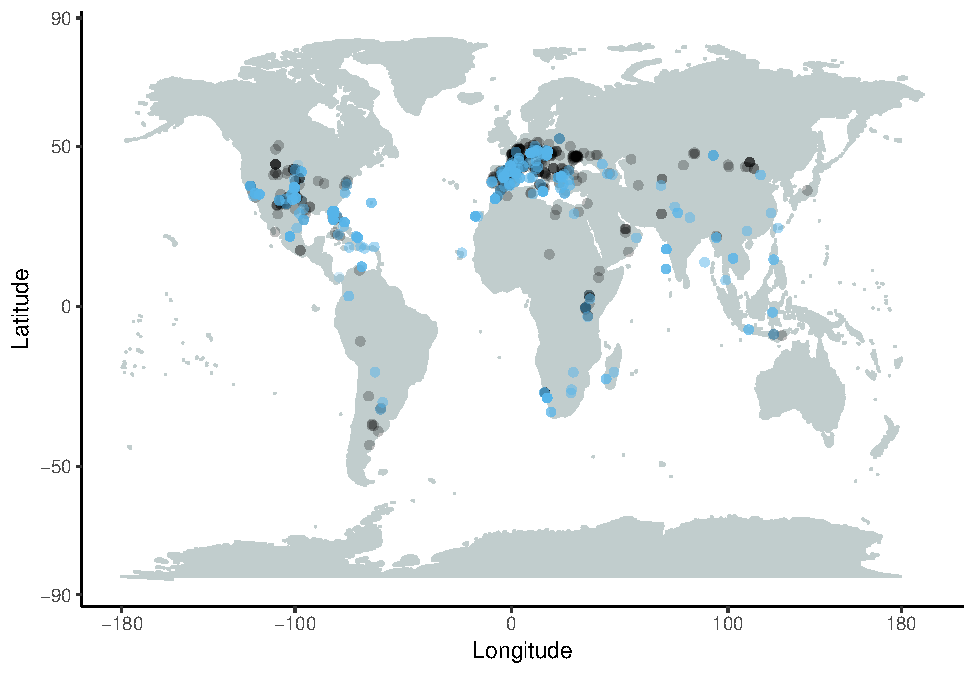
\includegraphics[width=0.7\textwidth]{MA_JJ_files/figure-latex/MapFossilOccurrences-1.pdf}
\end{center}

%\includegraphics[height=5 cm]<4-5>{pics/mm2.png}
%\includegraphics[height=5 cm]<6>{pics/mm3.png}
%\includegraphics[height=5 cm]<7->{pics/mm4.png}

%}
%\put(20,190){
%\fbox{
%\begin{minipage}[t]{0.5\linewidth}
\begin{itemize} %[<+->]
\p<1-> occurrences (black): 796 individuals, 647 localitis (Eocene - recent)
\bigskip
\p<2-> body size data (blue): 376 individuals, 193 localities (Miocene - recent)
\bigskip
\p<3-> of those: 106 from FosFarBase
\end{itemize}
%\end{minipage}}
%}

%\end{picture}
\end{frame}


% body size data: estimations etc.
\begin{frame}{Carapace length measurements/estimations}
%\begin{picture}(300,250)
%\put(170,80){
%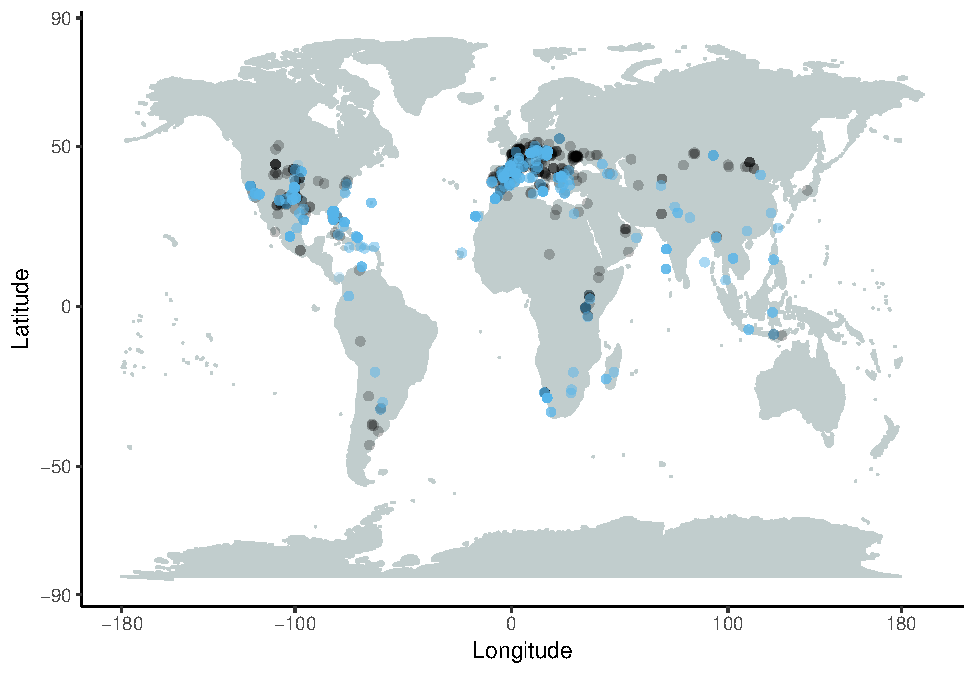
\includegraphics[width=0.7\textwidth]{MA_JJ_files/figure-latex/MapFossilOccurrences-1.pdf}
%\includegraphics[height=5 cm]<4-5>{pics/mm2.png}
%\includegraphics[height=5 cm]<6>{pics/mm3.png}
%\includegraphics[height=5 cm]<7->{pics/mm4.png}

%}
%\put(20,190){
%\fbox{
%\begin{minipage}[t]{0.5\linewidth}
\begin{itemize} %[<+->]
	\p<1-> exact measurements or estimations by original authors (n=...)
	\bigskip
	\p<2-> estimations from CL/PL ratio (--> extant measurements)
	\bigskip
	\p<3-> estimations from humeri/femora length, others (claw phalanges, verbal desription etc.)
\end{itemize}
%\end{minipage}}
%}

%\end{picture}
\end{frame}

% body size data: estimations etc.
\begin{frame}{Methods}
%\begin{picture}(300,250)
%\put(170,80){
%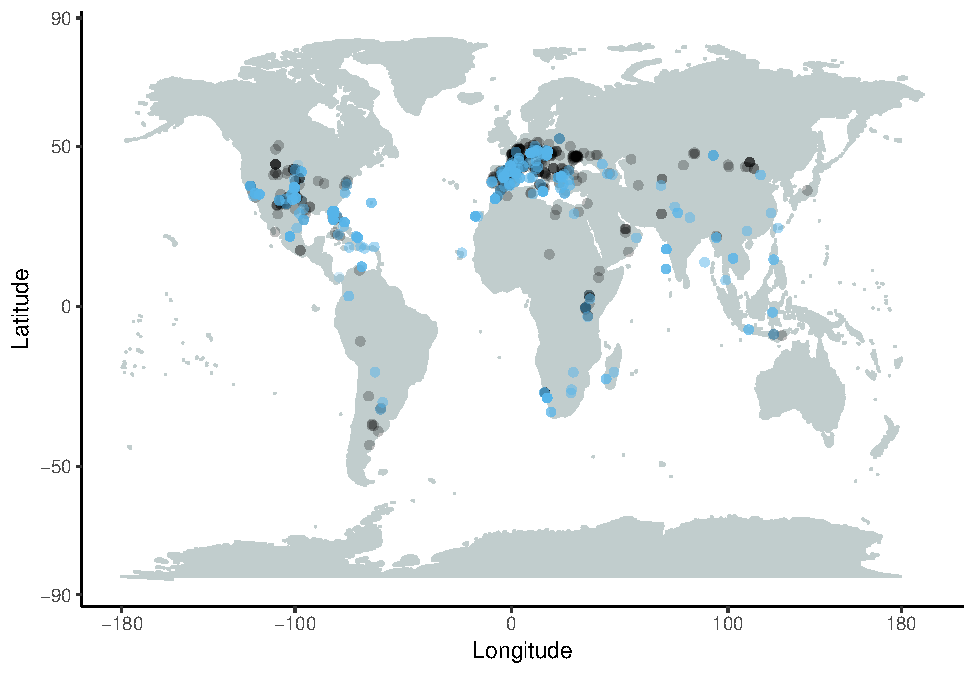
\includegraphics[width=0.7\textwidth]{MA_JJ_files/figure-latex/MapFossilOccurrences-1.pdf}
%\includegraphics[height=5 cm]<4-5>{pics/mm2.png}
%\includegraphics[height=5 cm]<6>{pics/mm3.png}
%\includegraphics[height=5 cm]<7->{pics/mm4.png}

%}
%\put(20,190){
%\fbox{
%\begin{minipage}[t]{0.5\linewidth}
\begin{itemize} %[<+->]
	\p<1-> SACs to check if sampling was sufficient --> generic level! add figure!!
	\bigskip
	\p<2-> histograms/density plots and boxplots (plus kruskal-wallis test, wilcoxon rank test)
	\bigskip
	\p<3-> paleoTS: fit different models to evolutionary trajectory of testudinid body size
\end{itemize}
%\end{minipage}}
%}

%\end{picture}
\end{frame}